\section{Modèle électronique}

%diapo 1
\begin{frame}
\frametitle{Modèle électronique}
\framesubtitle{Pourquoi une réalisation analogique ?}
\begin{itemize}
  \item \alert{Objectif :} observer physiquement les oscillations (cycle limite) du FHN.
  \item \alert{Problème :} la cubique \(v - \frac{v^3}{3}\) n’est pas directement réalisable avec des composants simples.
  \item \alert{Solution :} remplacer la cubique par une approximation linéaire par morceaux à 3 segments.
\end{itemize}
\vspace{0.3cm}
\alert{\textbf{Principe de l’approximation}}
\begin{itemize}
  \item On utilise une fonction affine par morceaux \(f(v)\) qui reproduit :
  \begin{itemize}
    \item une pente négative pour \(|v|\) petit 
    \item des pentes positives pour \(|v|\) grand 
  \end{itemize}
  \item Le circuit électronique est réalisable par des amplificateurs opérationnels.
\end{itemize}
\vspace{0.3cm}
\end{frame}

%Diapo2
\begin{frame}
\frametitle{Modèle électronique}
\framesubtitle{Principe du générateur de courant non linéaire}

\begin{block}{Rôle de la saturation}
La saturation de l'amplificateur opérationnel crée deux ruptures de pente dans la caractéristique \(I(V_2)\), permettant d'obtenir une approximation linéaire par morceaux de la non-linéarité cubique du modèle de FitzHugh--Nagumo.
\end{block}
\vspace{0.1cm}
\begin{columns}[T]
\column{0.5\textwidth}
\small
\[
h(V_{2})=
\begin{cases}
V_{+}
& \text{si } V_{2}>V_* \\[6pt]
\left(1+\dfrac{R_1}{R_2}\right)V_{2}
& \text{si } -V_*<V_{2}<V_* \\[6pt]
V_{-}
& \text{si } V_{2}< -V_*
\end{cases}
\]
\[
\text{où : }  V_*=\dfrac{R_2}{R_1+R_2}\,V_{\mathrm{sat}}
\]
\[
\text{on a alors : } I=\frac{V_2-h(V_2)}{R_3} = -f(V_{2}) 
\]
\column{0.5\textwidth}
\centering
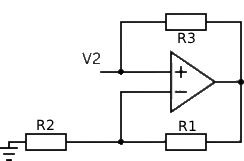
\includegraphics[width=\linewidth]{Figures/circuit.png}
\end{columns}
\end{frame}

%Diapo3
\begin{frame}
\frametitle{Modèle électronique}
\framesubtitle{Approximation linéaire par morceaux de la cubique}
\centering
\begin{figure}
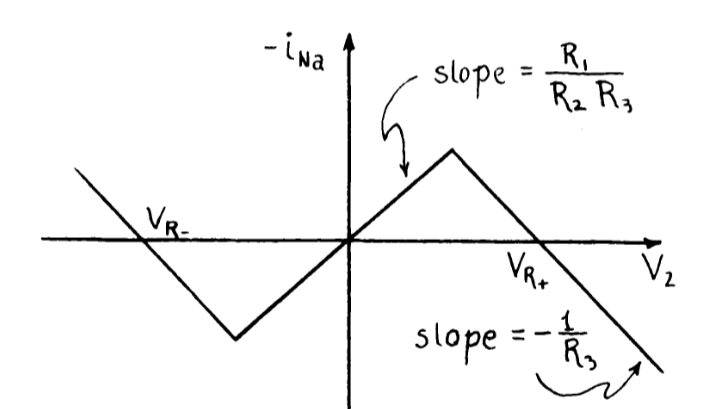
\includegraphics[scale = 0.4]{Figures/Linear_response.png}
\caption{Modèle linéaire}
%\source{James P.Keener, Analog Circuitry for the van der Pol and FitzHugh-Nagumo Equations}
\end{figure}
\vspace{0.3cm}
\end{frame}

%diapo4
\begin{frame}
\frametitle{Modèle électronique}
\framesubtitle{Inductance simulée par circuit à résistance négative}

\begin{block}{Rôle de l'inductance simulée}
L'association des composants passifs et de l'amplificateur opérationnel permet de synthétiser un comportement inductif sans utiliser de bobine réelle. 
\end{block}

\begin{columns}[T]
\column{0.5\textwidth}
\vspace{1.2cm}
\begin{equation}
\boxed{
C_2 R_5 R_4 \frac{di_2}{dt} + R_5\, i_2 = v - v_0
}
\end{equation}
%\[
%C_1 \frac{dv}{dt} = i_0 - f(v) - i_2\left(1 - \frac{R_5}{R_4}\right) - \frac{v - v_0}{R_4}
%\]

\centering

\column{0.5\textwidth}
\centering
\begin{figure}
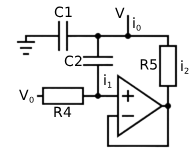
\includegraphics[scale = 0.6]{Figures/circuit1.png}
\caption{Schéma du montage à inductance simulée}
\end{figure}
\end{columns}


\end{frame}

%diapo5
\begin{frame}
\frametitle{Modèle électronique}
\framesubtitle{Circuit complet et équations du système}

\begin{block}{Circuit complet}
On monte un montage suiveur à un potentiomètre pour régler la tension d'entrée \(v_0\), 
suivi par l'inducteur simulé, et enfin le générateur de courant non linéaire réalisant la caractéristique \(f(v)\).
\end{block}

\vspace{0.1cm}

\begin{columns}[T]
\column{0.5\textwidth}
\small
\begin{equation}
\boxed{C_2 R_4 R_5 \frac{di_2}{dt} + R_5 i_2 = v - v_0}
\end{equation}
\nonumber
\vspace{0.3cm}
\begin{equation}
\boxed{C_1 \frac{dv}{dt} = i_0 - f(v) - i_2\left(1 - \frac{R_5}{R_4}\right) - \frac{v - v_0}{R_4}}
\end{equation}
\vspace{0.2cm}
\centering
\textit{(Équations du système analogue à FHN)}

\column{0.5\textwidth}
\centering
\begin{figure}
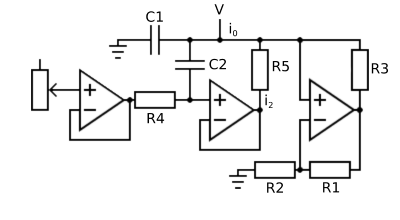
\includegraphics[width=\linewidth]{Figures/circuit_complet.png}
\caption{Schéma complet du modèle}
\end{figure}
\end{columns}
\end{frame}

\begin{frame}
\frametitle{Modèle électronique}
\framesubtitle{Allure prédite pour un modèle linéaire}

\begin{figure}
  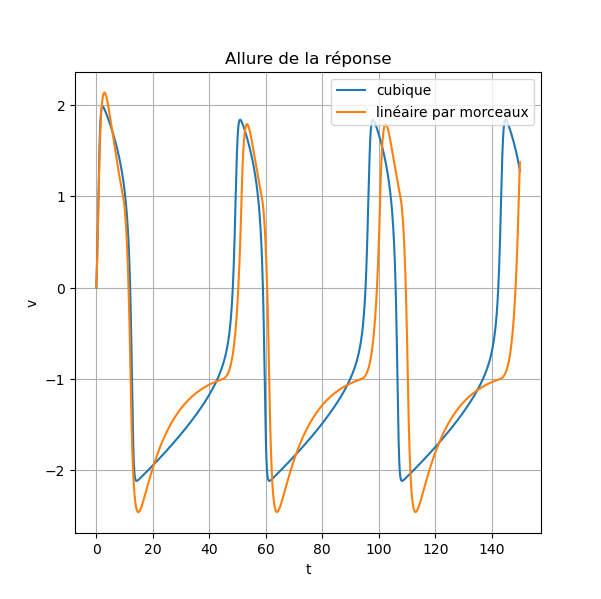
\includegraphics[scale = 1]{Figures/Linéaire.png}
  \caption{comparaison entre modèle linéaire par morceaux et modèle avec cubique}


